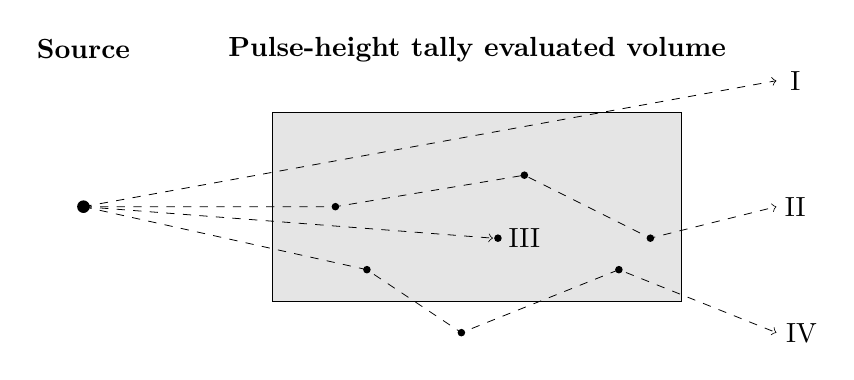
\begin{tikzpicture}[scale=0.8]
 
  % source
  \fill[black] (-5, 0) circle (0.1cm);
  \node[] at (-5, 2.5) {\textbf{Source}};
  
  % pht cell
  \fill[black!10] (-2, -1.5) -- (-2, 1.5) -- (4.5, 1.5) -- (4.5, -1.5) -- cycle;
  \draw [-, black, line width=0.1mm] (-2, -1.5) -- (-2, 1.5) -- (4.5, 1.5) -- (4.5, -1.5) -- cycle;
  \node[] at (1.25, 2.5) {\textbf{Pulse-height tally evaluated volume}};
  
  % particle tracks
  \draw[->, dashed, line width=0.1mm] (-5,0) -- (6, 2.0); 
  \draw[->, dashed, line width=0.1mm] (-5,0) -- (-1, 0) -- (2, 0.5) -- (4, -0.5) -- (6, 0); 
  \draw[->, dashed, line width=0.1mm] (-5,0) -- (1.5, -0.5); 
  \draw[->, dashed, line width=0.1mm] (-5,0) -- (-0.5, -1) -- (1, -2) -- (3.5, -1.0) -- (6, -2.0); 
  
  \fill[black] (-1, 0) circle (0.06cm);
  \fill[black] (2, 0.5) circle (0.06cm);
  \fill[black] (4, -0.5) circle (0.06cm);
  \fill[black] (1.58, -0.5) circle (0.06cm);
  \fill[black] (-0.5, -1) circle (0.06cm);
  \fill[black] (1, -2) circle (0.06cm);
  \fill[black] (3.5, -1) circle (0.06cm);
  
  % name particle tracks / particles
  \node[] at (6.3, 2.0) {I};
  \node[] at (6.3, 0) {II};
  \node[] at (2.0, -0.5) {III};
  \node[] at (6.4, -2.0) {IV};

\end{tikzpicture}
